\documentclass[11pt,a4paper]{article}
\usepackage[margin=21mm,top=21mm,bottom=21mm]{geometry}
\usepackage[T1]{fontenc}
\usepackage{lmodern,amsmath,amssymb,mathtools,tikz,fancyhdr,microtype}
\usepackage{needspace}
\usetikzlibrary{arrows.meta,calc,positioning}
\definecolor{DeepBlue}{HTML}{17365D}
\definecolor{MidBlue}{HTML}{2F75B5}
\definecolor{Orange}{HTML}{E79032}
\definecolor{Green}{HTML}{316645}
\definecolor{Red}{HTML}{B33738}
\definecolor{Ink}{HTML}{1C2B38}
\color{Ink}
\pagestyle{fancy}\fancyhf{}
\fancyhead[L]{\small\sffamily\color{DeepBlue}Quantics tensor networks}
\fancyhead[R]{\small\sffamily\color{DeepBlue}Simplex integration}
\fancyfoot[R]{\small\sffamily\thepage}
\renewcommand{\headrulewidth}{0.3pt}
\setlength{\headheight}{15pt}
\setlength{\parindent}{0pt}\setlength{\parskip}{5pt}
\raggedbottom
\newcommand{\titleline}[1]{\par\Needspace{7\baselineskip}\medskip{\LARGE\sffamily\bfseries\color{DeepBlue}#1\par}\vspace{3pt}}
\newcommand{\subhead}[1]{\par\Needspace{4\baselineskip}\smallskip{\large\sffamily\bfseries\color{DeepBlue}#1\par}}
\newcommand{\note}[1]{{\small #1\par}}
\newcommand{\ind}{\mathbf 1}
\tikzset{
 bond/.style={draw=DeepBlue,line width=1.05pt},
 phys/.style={draw=Red,line width=1.1pt},
 core/.style={circle,draw=MidBlue,fill=MidBlue!12,thick,minimum size=7mm,inner sep=1pt},
 junction/.style={rounded corners=2pt,draw=DeepBlue,fill=DeepBlue!10,thick,minimum width=12mm,minimum height=7mm},
 oper/.style={rounded corners=1.5pt,draw=Orange!75!black,fill=Orange!22,thick,minimum width=10mm,minimum height=7mm},
 msg/.style={rounded corners=2pt,draw=Green,fill=Green!12,thick,minimum width=11mm,minimum height=7mm},
 go/.style={-{Stealth[length=2.5mm]},draw=DeepBlue,line width=1.1pt},
 lab/.style={font=\small,inner sep=2pt}, each/.style={font=\small}
}
% A grouped contraction: top legs carry tree indices, bottom legs carry time registers.
% Arguments: gap branch, old message, their bonds, tree tensor, surviving bond, result.
\newcommand{\mergepic}[7]{\begin{tikzpicture}[x=1cm,y=.82cm,each,baseline=(current bounding box.center)]
 \node[core] (k) at (0,0) {$#1$}; \node[msg] (v) at (3,0) {$#2$};
 \node[junction] (j) at (1.5,.95) {$#5$}; \node[oper] (z) at (1.5,-.95) {$T$};
 \draw[bond] (k)--node[above left,lab] {$#3$} (j);
 \draw[bond] (v)--node[above right,lab] {$#4$} (j);
 \draw[bond] (j)--++(0,.77) node[above,lab] {$#6$};
 \draw[bond] (k)--node[below left,lab] {$n$} (z);
 \draw[bond] (v)--node[below right,lab] {$m$} (z);
 \draw[phys] (z)--++(0,-.55) node[below,lab] {$m'$};
 \draw[go] (3.9,0)--(5.0,0);
 \node[msg] (o) at (6,0) {$#7$};
 \draw[bond] (o)--++(0,.8) node[above,lab] {$#6$};
 \draw[phys] (o)--++(0,-.8) node[below,lab] {$m'$};
 \end{tikzpicture}}
\begin{document}
\titleline{Retracting a four-gap tensor tree}
The goal is a single MPS whose open physical legs encode the observation time \(t\).
The input has four branches for \(v_i=u_{i-1}-u_i\), where \(u_0=t\), and two
internal tensors \(L^{(8)}\) and \(R^{(9)}\). We take \(\lambda=1\) throughout.

\par\noindent\begin{minipage}{\linewidth}
\begin{center}
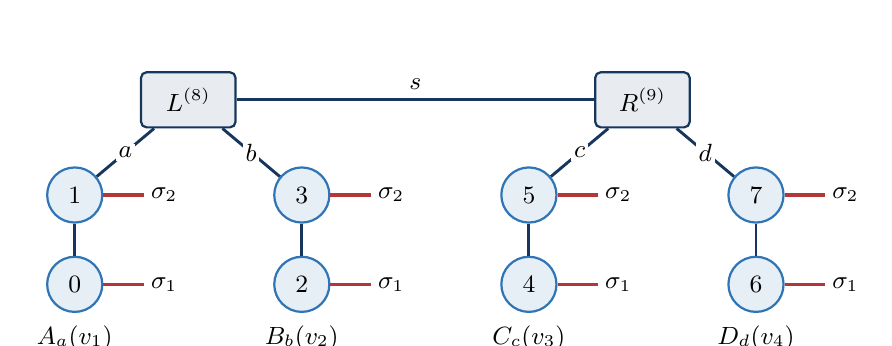
\begin{tikzpicture}[x=1.03cm,y=.93cm,each]
 \node[junction] (l) at (1.4,2) {$L^{(8)}$}; \node[junction] (r) at (7,2) {$R^{(9)}$};
 \draw[bond] (l)--node[above] {$s$} (r);
 \foreach \x/\lo/\hi/\f/\i/\ch/\parent in
 {0/0/1/A/1/a/l,2.8/2/3/B/2/b/l,5.6/4/5/C/3/c/r,8.4/6/7/D/4/d/r}{
   \node[core] (hi\i) at (\x,.7) {\hi};
   \node[core] (lo\i) at (\x,-.52) {\lo};
   \draw[bond] (lo\i)--(hi\i);
   \draw[bond] (hi\i)--node[midway,fill=white,inner sep=1pt] {$\ch$} (\parent);
   \draw[phys] (lo\i.east)--++(.5,0) node[right,lab] {$\sigma_1$};
   \draw[phys] (hi\i.east)--++(.5,0) node[right,lab] {$\sigma_2$};
   \node at (\x,-1.25) {$\f_{\ch}(v_{\i})$};
 }
\end{tikzpicture}
\end{center}
\note{Each numbered circle is one bit site. A red stub is an open physical index.
The two-bit illustration assigns the most significant bit to the even site and the
least significant bit to the odd site. With \(p\) bits, replace each pair by its \(p\)-site chain.}
\end{minipage}\par

\[
 F(v_1,v_2,v_3,v_4)=\sum_{a,b,c,d,s}
 A_a(v_1)B_b(v_2)L^{(8)}_{abs}R^{(9)}_{scd}C_c(v_3)D_d(v_4).
\]
\subhead{0.1\quad Identify the gap registers and their domain}
The integration variables are the ordered times \(0\le u_4\le u_3\le u_2\le u_1\le t\).
The TPS takes their successive differences as its arguments:
\[
 Q_4(t)=\int_0^t\!\mathrm{d}u_1\int_0^{u_1}\!\mathrm{d}u_2
 \int_0^{u_2}\!\mathrm{d}u_3\int_0^{u_3}\!\mathrm{d}u_4\,
 F(t-u_1,\,u_1-u_2,\,u_2-u_3,\,u_3-u_4).
\]
With \(u_0=t\), set \(v_i=u_{i-1}-u_i\). This change of variables has
unit absolute Jacobian and gives the gap simplex \(v_i\ge0\), \(\sum_i v_i\le t\).
The remaining times that bound the successive gap integrations are
\[
\begin{aligned}
 u_1 &= t-v_1,\\
 u_2 &= u_1-v_2=(t-v_1)-v_2=t-(v_1+v_2),\\
 u_3 &= u_2-v_3=\bigl((t-v_1)-v_2\bigr)-v_3=t-(v_1+v_2+v_3).
\end{aligned}
\]
\subhead{0.2\quad Choose the order of elimination}
Read these integrals from the inside out. The upper limit on branch \(67\)
is \(u_3=t-(v_1+v_2+v_3)\). We keep this limit as a binary register while removing
the branch. Each subsequent contraction passes the register to its parent:
\[
 \underbrace{D_d(v_4)}_{67}
 \ \longrightarrow\ M_d(u_3)
 \ \xrightarrow{\ 45,\;9\ }\ N_s(u_2)
 \ \xrightarrow{\ 23,\;8\ }\ P_a(u_1)
 \ \xrightarrow{\ 01\ }\ Q_4(t).
\]
One input tree yields this whole function of \(t\) when its gap kernels
are common throughout the observation window.

\titleline{6. The four-gap TPS and its simplex integral}
\[
 f(v_1,v_2,v_3,v_4)
 =\sum_{a,b,c,d,s}
 A_a(v_1)\,B_b(v_2)\,L^{(8)}_{abs}\,R^{(9)}_{scd}\,C_c(v_3)\,D_d(v_4).
\]
Our objective is the integral over the ordered times \(0\le u_4\le u_3\le u_2\le u_1\le t\).
The four branches of the TPS take successive time differences as their arguments:
\[
 Q_4(t)=
 \int_0^t\!\mathrm{d}u_1
 \int_0^{u_1}\!\mathrm{d}u_2
 \int_0^{u_2}\!\mathrm{d}u_3
 \int_0^{u_3}\!\mathrm{d}u_4\;
 f(t-u_1,\,u_1-u_2,\,u_2-u_3,\,u_3-u_4).
\]
\subhead{6.1\quad Integrate the ordered times recursively}
Starting with the innermost time \(u_4\), define
\[
\begin{aligned}
 \psi_{4,d}(u_3)
   &=\int_0^{u_3}\!\mathrm{d}u_4\,D_d(u_3-u_4),\\[3pt]
 \psi_{3,s}(u_2)
   &=\sum_{c,d}R^{(9)}_{scd}\int_0^{u_2}\!\mathrm{d}u_3\,
     C_c(u_2-u_3)\,\psi_{4,d}(u_3),\\[3pt]
 \psi_{2,a}(u_1)
   &=\sum_{b,s}L^{(8)}_{abs}\int_0^{u_1}\!\mathrm{d}u_2\,
     B_b(u_1-u_2)\,\psi_{3,s}(u_2),\\[3pt]
 \psi_1(t)
   &=\sum_a\int_0^t\!\mathrm{d}u_1\,
     A_a(t-u_1)\,\psi_{2,a}(u_1)=Q_4(t).
\end{aligned}
\]
The three intermediate functions are the messages \(M_d\), \(N_s\), and \(P_a\)
in Section 0.2, respectively.

\subhead{6.2\quad Construct \(\psi_{4,d}(u_3)\) by summing over \(u_4\)}
Let \(R\) be the number of bits in each of the \(v_4\), \(u_4\), and \(u_3\) registers.
Write \(v_4=kh\), \(u_4=mh\), \(u_3=nh\), and \(D_d[k]=D_d(kh)\), with \(h=\Delta x\).
Each index ranges from \(0\) to \(2^R-1\). Number the bits from least to most significant,
so \(m=\sum_{j=1}^{R}2^{j-1}m_j\), with the same ordering for \(k\) and \(n\).
\[
\begin{aligned}
 \psi_{4,d}(u_3)
 &=\int_0^{u_3}D_d(u_3-u_4)\,\mathrm{d}u_4\\
 &\approx h\sum_{m=0}^{n}D_d\bigl((n-m)h\bigr)\\
 &=h\sum_{m_1=0}^{1}\cdots\sum_{m_R=0}^{1}
       \sum_{k=0}^{2^R-1}\delta_{n,k+m}\,D_d[k].
\end{aligned}
\]
Each bit sum contracts one \(u_4\) leg with \((1,1)\).

\textbf{1. Use \(S\) to form the difference.}
Contract the \(k\) register of \(D_d[k]=D_d(kh)\) with
\(S_{n,k,m}=\delta_{n,k+m}\), using ordinary integer addition with zero
boundary carries. The resulting MPO has an upper-time register \(n\) and
an integration register \(m\):
\[
 \mathcal D_d[n,m]=\sum_k S_{n,k,m}D_d[k]
 =\begin{cases}D_d((n-m)h),&m\le n,\\0,&m>n.\end{cases}
\]

\textbf{2. Sum every \(u_4\) bit.}
Attach \(e=(1,1)\) to each physical leg \(m_j\) of the MPO. Both bit
values enter with weight one. Leave every \(n_j\) leg and the tree bond \(d\) open.
\[
 Y_d[n]=\sum_{m_1,\ldots,m_R}\mathcal D_d[n,m]\prod_{j=1}^{R}e_{m_j}
       =\sum_{m=0}^{n} D_d((n-m)h).
\]
\begin{center}
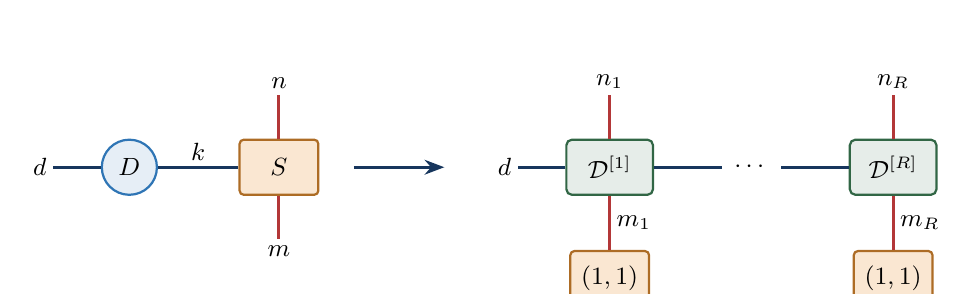
\begin{tikzpicture}[each]
 \node[core] (D) at (0,0) {$D$};
 \node[oper] (S) at (1.9,0) {$S$};
 \draw[bond] (D.west)--++(-.6,0) node[left,lab] {$d$};
 \draw[bond] (D.east)--node[above,lab] {$k$} (S.west);
 \draw[phys] (S.north)--++(0,.55) node[above,lab] {$n$};
 \draw[phys] (S.south)--++(0,-.55) node[below,lab] {$m$};
 \draw[go] (2.85,0)--(4,0);
 \node[msg] (lo) at (6.1,0) {$\mathcal D^{[1]}$};
 \node[msg] (hi) at (9.7,0) {$\mathcal D^{[R]}$};
 \draw[bond] (lo.west)--++(-.6,0) node[left,lab] {$d$};
 \draw[bond] (lo.east)--(7.52,0); \node at (7.9,0) {$\cdots$};
 \draw[bond] (8.28,0)--(hi.west);
 \foreach \site/\bit in {lo/1,hi/R} {
   \draw[phys] (\site.north)--++(0,.55) node[above,lab] {$n_{\bit}$};
   \node[oper] (e\site) at ($(\site.south)+(0,-1.05)$) {$(1,1)$};
   \draw[phys] (\site.south)--node[right,lab] {$m_{\bit}$} (e\site.north);
 }
\end{tikzpicture}
\end{center}
\note{Left: contract the gap register \(k\) with \(S\). Right: the resulting
MPO cores each receive one vector on their \(u_4\) leg. This contraction gives
the unweighted row sum \(Y_d[n]\).}

\textbf{3. Weight the inclusive sum.}
The subtractor enforces \(n=m+k\) with \(k\ge 0\), so the allowed rows and
columns satisfy \(0\le m\le n\). Equality corresponds to the allowed gap
\(k=0\). Contracting the \(u_4\) bits includes this term automatically.
Multiply the resulting row sum by \(h=\Delta x\) once:
\[
 \boxed{\psi_{4,d}^{(h)}[n]=hY_d[n]
       =h\sum_{m=0}^{n}\mathcal D_d[n,m].}
\]
The \(u_3\) register and tree bond \(d\) remain open.

\par\noindent\begin{minipage}{\linewidth}
\textbf{Full tree before and after the \(u_4\) contraction.}
\begin{center}
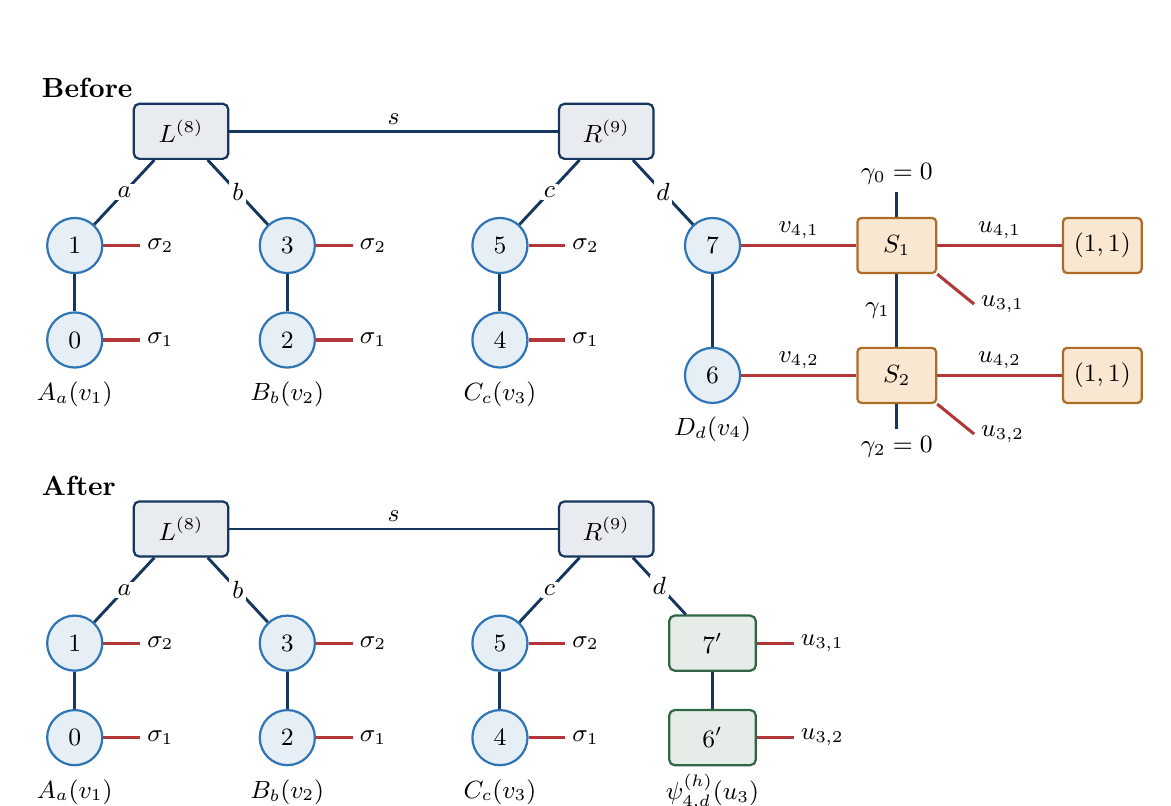
\begin{tikzpicture}[each,x=.90cm]
 \foreach \panel/\offset in {0/0,1/-5.05}{
 \begin{scope}[yshift=\offset cm]
 \node[junction] (left) at (1.5,2.1) {$L^{(8)}$};
 \node[junction] (right) at (7.5,2.1) {$R^{(9)}$};
 \draw[bond] (left)--node[above,lab] {$s$} (right);
 \foreach \x/\topsite/\bottomsite/\branch/\idx/\leg/\parent in
   {0/1/0/A/1/a/left,3/3/2/B/2/b/left,6/5/4/C/3/c/right}{
   \node[core] (t\idx) at (\x,.65) {$\topsite$};
   \node[core] (b\idx) at (\x,-.55) {$\bottomsite$};
   \draw[bond] (t\idx)--node[midway,fill=white,inner sep=1pt] {$\leg$} (\parent);
   \draw[bond] (t\idx)--(b\idx);
   \draw[phys] (t\idx.east)--++(.52,0) node[right,lab] {$\sigma_2$};
   \draw[phys] (b\idx.east)--++(.52,0) node[right,lab] {$\sigma_1$};
   \node at (\x,-1.24) {$\branch_{\leg}(v_{\idx})$};
 }
 \ifnum\panel=0
 \node[anchor=west,font=\bfseries] at (-.6,2.65) {Before};
 \foreach \j/\y/\site in {1/.65/7,2/-1.0/6}{
   \node[core] (D\j) at (9,\y) {$\site$};
   \node[oper] (S\j) at (11.6,\y) {$S_{\j}$};
   \node[oper] (E\j) at (14.5,\y) {$(1,1)$};
   \draw[phys] (D\j.east)--node[above,lab] {$v_{4,\j}$} (S\j.west);
   \draw[phys] (S\j.east)--node[above,lab] {$u_{4,\j}$} (E\j.west);
   \draw[phys] (S\j.south east)--++(.52,-.38) node[right,lab] {$u_{3,\j}$};
 }
 \draw[bond] (right)--node[midway,fill=white,inner sep=1pt] {$d$} (D1);
 \draw[bond] (D1)--(D2);
 \draw[bond] (S1.north)--++(0,.32) node[above,lab] {$\gamma_0=0$};
 \draw[bond] (S1.south)--node[left,lab] {$\gamma_1$} (S2.north);
 \draw[bond] (S2.south)--++(0,-.32) node[below,lab] {$\gamma_2=0$};
 \node at (9,-1.68) {$D_d(v_4)$};
 \else
 \node[anchor=west,font=\bfseries] at (-.6,2.65) {After};
 \node[msg] (p1) at (9,.65) {$7'$};
 \node[msg] (p2) at (9,-.55) {$6'$};
 \draw[bond] (p1)--node[midway,fill=white,inner sep=1pt] {$d$} (right);
 \draw[bond] (p1)--(p2);
 \draw[phys] (p1.east)--++(.52,0) node[right,lab] {$u_{3,1}$};
 \draw[phys] (p2.east)--++(.52,0) node[right,lab] {$u_{3,2}$};
 \node at (9,-1.24) {$\psi_{4,d}^{(h)}(u_3)$};
 \fi
 \end{scope}
 }
\end{tikzpicture}
\end{center}
\note{Each adder core \(S_j\) receives a gap bit \(v_{4,j}\) from site \(7\) or \(6\).
The two \((1,1)\) vectors sum the \(u_4\) bits, and the carry \(\gamma_1\) links the adders.
Contracting this branch and multiplying by \(h\) once gives \(\psi_{4,d}^{(h)}(u_3)\).
Its open legs encode \(u_3=h(u_{3,1}+2u_{3,2})\), and bond \(d\) connects it to node \(9\).
With \(R\) bits the branch has \(R\) open \(u_3\) legs.}
\end{minipage}\par

\subhead{6.3\quad Express \(\psi_{3,s}(u_2)\) in terms of \(\psi_{4,d}(u_3)\)}
Write \(u_2=nh\), \(u_3=mh\), \(v_3=kh\), and \(C_c[k]=C_c(kh)\).
All three registers have \(R\) bits. Here \(m=\sum_{j=1}^R2^{j-1}m_j\)
indexes the output of Section 6.2. Using the same inclusive grid sum gives
\[
\begin{aligned}
 \psi_{3,s}(u_2)
 &=\sum_{c,d}R^{(9)}_{scd}\int_0^{u_2}
 C_c(u_2-u_3)\,\psi_{4,d}(u_3)\,\mathrm{d}u_3\\
 &\approx h\sum_{c,d}R^{(9)}_{scd}\sum_{m=0}^{n}
 C_c\bigl((n-m)h\bigr)\,\psi_{4,d}^{(h)}[m]\\
 &= h\sum_{c,d}R^{(9)}_{scd}
 \sum_{m_1=0}^1\cdots\sum_{m_R=0}^1\sum_{k=0}^{2^R-1}
 \delta_{n,k+m}\,C_c[k]\,\psi_{4,d}^{(h)}[m].
\end{aligned}
\]

\textbf{1. Form the two-time MPO.}
Contract the \(v_3\) register of \(C_c\) with the same subtractor \(S\) as in Section 6.2:
\[
 C'_c[n,m]=\sum_{k=0}^{2^R-1}\delta_{n,k+m}\,C_c[k]
 =\begin{cases} C_c((n-m)h),&m\le n,\\0,&m>n.\end{cases}
\]
Ordinary integer addition enforces \(u_3\le u_2\), including \(u_3=u_2\).

\textbf{2. Connect the matching \(u_3\) legs.}
For each \(j\), join leg \(m_j\) of \(C'_c\) directly to leg \(m_j\) of
\(\psi_{4,d}^{(h)}\). Each wire sums over its two bit values. Together the wires give
\[
 X_{cd}^{(h)}[n]=h\sum_{m=0}^{2^R-1}C'_c[n,m]\,\psi_{4,d}^{(h)}[m].
\]
The factor \(h\) weights this integration over \(u_3\) once.

\begin{center}
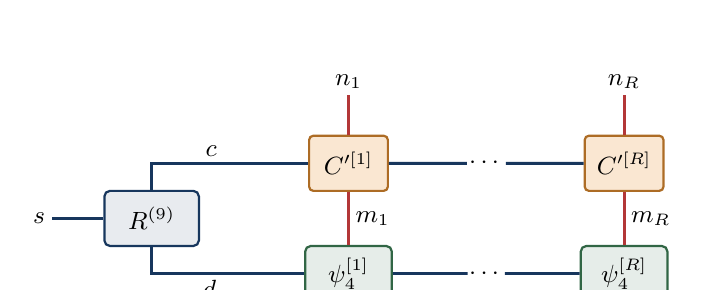
\begin{tikzpicture}[each]
 \node[junction] (r) at (0,0) {$R^{(9)}$};
 \draw[bond] (r.west)--++(-.65,0) node[left,lab] {$s$};
 \foreach \x/\j in {2.5/1,6/R} {
   \node[oper] (c\j) at (\x,.7) {$C'^{[\j]}$};
   \node[msg] (p\j) at (\x,-.7) {$\psi_4^{[\j]}$};
   \draw[phys] (c\j.south)--node[right,lab] {$m_{\j}$} (p\j.north);
   \draw[phys] (c\j.north)--++(0,.5) node[above,lab] {$n_{\j}$};
 }
 \draw[bond] (r.north)|-node[above,pos=.69,lab] {$c$} (c1.west);
 \draw[bond] (r.south)|-node[below,pos=.69,lab] {$d$} (p1.west);
 \foreach \a in {c,p}{
   \draw[bond] (\a1.east)--($(\a1.east)!.40!(\a R.west)$);
   \path (\a1.east)--node[midway] {$\cdots$} (\a R.west);
   \draw[bond] ($(\a1.east)!.60!(\a R.west)$)--(\a R.west);
 }
\end{tikzpicture}
\end{center}

\textbf{3. Contract node 9.}
The existing tree node joins the \(c\) and \(d\) bonds. The open legs are the
\(u_2\) bits \(n_1,\ldots,n_R\) and the tree bond \(s\):
\[
 \boxed{\psi_{3,s}^{(h)}[n]=\sum_{c,d}R^{(9)}_{scd}\,X_{cd}^{(h)}[n].}
\]
\par\noindent\begin{minipage}{\linewidth}
\textbf{Full tree before and after the \(u_3\) contraction.}
\begin{center}
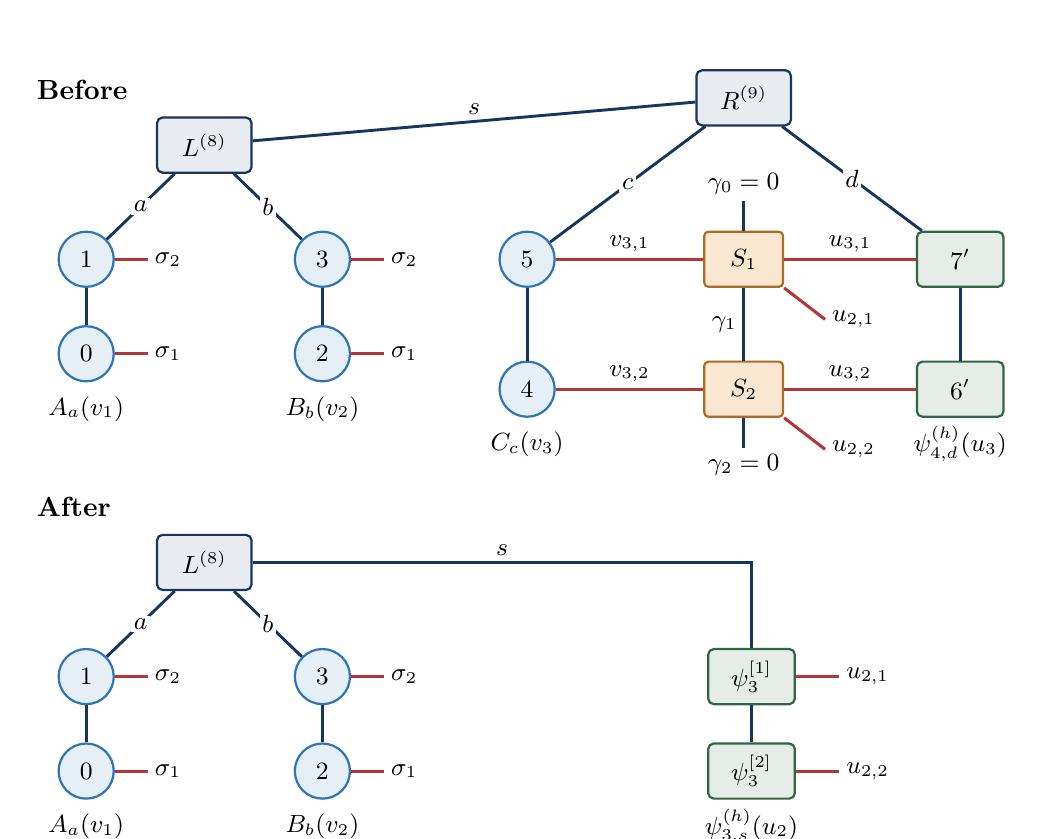
\begin{tikzpicture}[each]
 \foreach \stage/\offset in {before/0,after/-5.3}{
  \begin{scope}[yshift=\offset cm]
   \node[junction] (L\stage) at (1.5,2.1) {$L^{(8)}$};
   \foreach \x/\topsite/\bottomsite/\branch/\idx/\leg in
     {0/1/0/A/1/a,3/3/2/B/2/b}{
    \node[core] (top\stage\idx) at (\x,.65) {$\topsite$};
    \node[core] (bottom\stage\idx) at (\x,-.55) {$\bottomsite$};
    \draw[bond] (top\stage\idx)--node[midway,fill=white,inner sep=1pt] {$\leg$} (L\stage);
    \draw[bond] (top\stage\idx)--(bottom\stage\idx);
    \draw[phys] (top\stage\idx.east)--++(.42,0) node[right,lab] {$\sigma_2$};
    \draw[phys] (bottom\stage\idx.east)--++(.42,0) node[right,lab] {$\sigma_1$};
    \node at (\x,-1.25) {$\branch_{\leg}(v_{\idx})$};
   }
  \end{scope}
 }
 \node[anchor=west,font=\bfseries] at (-.75,2.8) {Before};
 \node[junction] (nine) at (8.35,2.7) {$R^{(9)}$};
 \draw[bond] (Lbefore)--node[above,lab] {$s$} (nine);
 \foreach \j/\y/\csite/\psite in {1/.65/5/7,2/-1.0/4/6}{
   \node[core] (c\j) at (5.6,\y) {$\csite$};
   \node[oper] (adder\j) at (8.35,\y) {$S_{\j}$};
   \node[msg] (p\j) at (11.1,\y) {$\psite'$};
   \draw[phys] (c\j.east)--node[above,lab] {$v_{3,\j}$} (adder\j.west);
   \draw[phys] (adder\j.east)--node[above,lab] {$u_{3,\j}$} (p\j.west);
   \draw[phys] (adder\j.south east)--++(.52,-.40) node[right,lab] {$u_{2,\j}$};
 }
 \draw[bond] (nine)--node[midway,fill=white,inner sep=1pt] {$c$} (c1);
 \draw[bond] (nine)--node[midway,fill=white,inner sep=1pt] {$d$} (p1);
 \draw[bond] (c1)--(c2); \draw[bond] (p1)--(p2);
 \draw[bond] (adder1.north)--++(0,.37) node[above,lab] {$\gamma_0=0$};
 \draw[bond] (adder1.south)--node[left,lab] {$\gamma_1$} (adder2.north);
 \draw[bond] (adder2.south)--++(0,-.38) node[below,lab] {$\gamma_2=0$};
 \node at (5.6,-1.7) {$C_c(v_3)$};
 \node at (11.1,-1.7) {$\psi_{4,d}^{(h)}(u_3)$};
 \begin{scope}[yshift=-5.3cm]
  \node[anchor=west,font=\bfseries] at (-.75,2.8) {After};
  \foreach \j/\y in {1/.65,2/-.55}{
    \node[msg] (out\j) at (8.45,\y) {$\psi_3^{[\j]}$};
    \draw[phys] (out\j.east)--++(.55,0) node[right,lab] {$u_{2,\j}$};
  }
  \draw[bond] (Lafter.east)--node[above,lab] {$s$} (8.45,2.1)--(out1.north);
  \draw[bond] (out1)--(out2);
  \node at (8.45,-1.25) {$\psi_{3,s}^{(h)}(u_2)$};
 \end{scope}
\end{tikzpicture}
\end{center}
\note{Sites \(5,4\) carry \(C_c(v_3)\). Each adder core \(S_j\) connects a \(v_{3,j}\) bit to the matching \(u_{3,j}\) bit of \(\psi_{4,d}^{(h)}\) and exposes the \(u_{2,j}\) bit. It enforces \(v_{3,j}+u_{3,j}+\gamma_{j-1}=u_{2,j}+2\gamma_j\). The internal carry \(\gamma_1\) passes from \(S_1\) to \(S_2\), with both boundary carries fixed to zero. Contracting this subtree with node \(9\) and weighting by \(h\) gives the lower tree.}
\end{minipage}\par
\Needspace{9\baselineskip}
\subhead{6.4\quad Express \(\psi_{2,a}(u_1)\) in terms of \(\psi_{3,s}(u_2)\)}
Write \(u_1=nh\), \(u_2=mh\), \(v_2=kh\), and \(B_b[k]=B_b(kh)\).
All three registers have \(R\) bits. Here \(m=\sum_{j=1}^R2^{j-1}m_j\)
indexes the output of Section 6.3. Using the same inclusive grid sum gives
\[
\begin{aligned}
 \psi_{2,a}(u_1)
 &=\sum_{b,s}L^{(8)}_{abs}\int_0^{u_1}
 B_b(u_1-u_2)\,\psi_{3,s}(u_2)\,\mathrm{d}u_2\\
 &\approx h\sum_{b,s}L^{(8)}_{abs}\sum_{m=0}^{n}
 B_b\bigl((n-m)h\bigr)\,\psi_{3,s}^{(h)}[m]\\
 &= h\sum_{b,s}L^{(8)}_{abs}
 \sum_{m_1=0}^1\cdots\sum_{m_R=0}^1\sum_{k=0}^{2^R-1}
 \delta_{n,k+m}\,B_b[k]\,\psi_{3,s}^{(h)}[m].
\end{aligned}
\]

\textbf{1. Form the two-time MPO.}
Contract the \(v_2\) register of \(B_b\) with the same subtractor \(S\) as in Section 6.3:
\[
 B'_b[n,m]=\sum_{k=0}^{2^R-1}\delta_{n,k+m}\,B_b[k]
 =\begin{cases} B_b((n-m)h),&m\le n,\\0,&m>n.\end{cases}
\]
Ordinary integer addition enforces \(u_2\le u_1\), including \(u_2=u_1\).

\textbf{2. Connect the matching \(u_2\) legs.}
For each \(j\), join leg \(m_j\) of \(B'_b\) directly to leg \(m_j\) of
\(\psi_{3,s}^{(h)}\). Each wire sums over its two bit values. Together the wires give
\[
 X_{bs}^{(h)}[n]=h\sum_{m=0}^{2^R-1}B'_b[n,m]\,\psi_{3,s}^{(h)}[m].
\]
The factor \(h\) weights this integration over \(u_2\) once.

\begin{center}
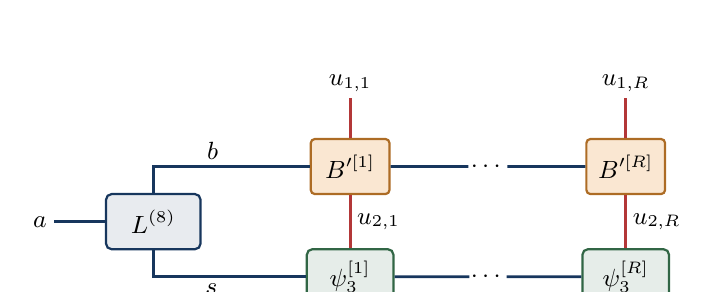
\begin{tikzpicture}[each]
 \node[junction] (r) at (0,0) {$L^{(8)}$};
 \draw[bond] (r.west)--++(-.65,0) node[left,lab] {$a$};
 \foreach \x/\j in {2.5/1,6/R} {
   \node[oper] (c\j) at (\x,.7) {$B'^{[\j]}$};
   \node[msg] (p\j) at (\x,-.7) {$\psi_3^{[\j]}$};
   \draw[phys] (c\j.south)--node[right,lab] {$u_{2,\j}$} (p\j.north);
   \draw[phys] (c\j.north)--++(0,.5) node[above,lab] {$u_{1,\j}$};
 }
 \draw[bond] (r.north)|-node[above,pos=.69,lab] {$b$} (c1.west);
 \draw[bond] (r.south)|-node[below,pos=.69,lab] {$s$} (p1.west);
 \foreach \a in {c,p}{
   \draw[bond] (\a1.east)--($(\a1.east)!.40!(\a R.west)$);
   \path (\a1.east)--node[midway] {$\cdots$} (\a R.west);
   \draw[bond] ($(\a1.east)!.60!(\a R.west)$)--(\a R.west);
 }
\end{tikzpicture}
\end{center}

\textbf{3. Contract node 8.}
The existing tree node joins the \(b\) and \(s\) bonds. The open legs are the
\(u_1\) bits \(n_1,\ldots,n_R\) and the tree bond \(a\):
\[
 \boxed{\psi_{2,a}^{(h)}[n]=\sum_{b,s}L^{(8)}_{abs}\,X_{bs}^{(h)}[n].}
\]
\par\noindent\begin{minipage}{\linewidth}
\textbf{Full tree before and after the \(u_2\) contraction.}
\begin{center}
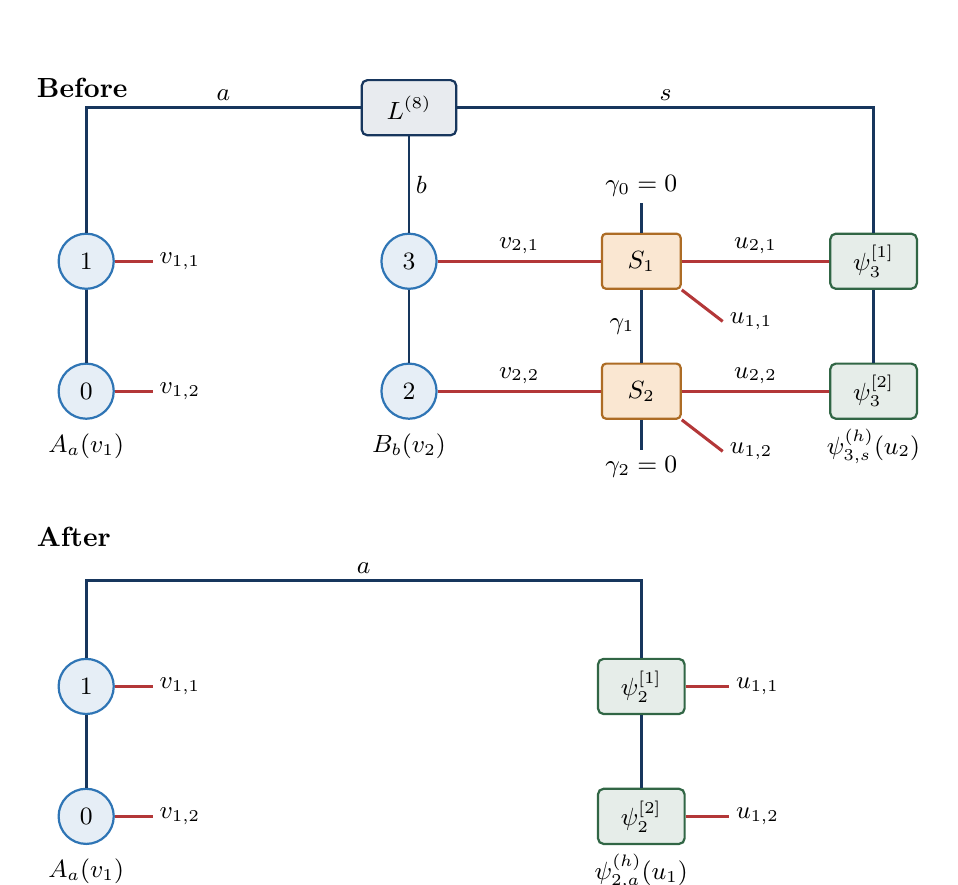
\begin{tikzpicture}[each]
 \foreach \stage/\shift in {before/0,after/-5.4}{
  \begin{scope}[yshift=\shift cm]
   \node[core] (Aone\stage) at (0,.65) {$1$};
   \node[core] (Azero\stage) at (0,-1) {$0$};
   \draw[bond] (Aone\stage)--(Azero\stage);
   \draw[phys] (Aone\stage.east)--++(.48,0) node[right,lab] {$v_{1,1}$};
   \draw[phys] (Azero\stage.east)--++(.48,0) node[right,lab] {$v_{1,2}$};
   \node at (0,-1.7) {$A_a(v_1)$};
  \end{scope}
 }
 \node[anchor=west,font=\bfseries] at (-.75,2.85) {Before};
 \node[junction] (eight) at (4.1,2.6) {$L^{(8)}$};
 \draw[bond] (eight.west)--node[above,lab] {$a$} (0,2.6)--(Aonebefore.north);
 \foreach \j/\y/\site in {1/.65/3,2/-1/2}{
   \node[core] (B\j) at (4.1,\y) {$\site$};
   \node[oper] (add\j) at (7.05,\y) {$S_{\j}$};
   \node[msg] (old\j) at (10,\y) {$\psi_3^{[\j]}$};
   \draw[phys] (B\j.east)--node[above,lab] {$v_{2,\j}$} (add\j.west);
   \draw[phys] (add\j.east)--node[above,lab] {$u_{2,\j}$} (old\j.west);
   \draw[phys] (add\j.south east)--++(.52,-.40) node[right,lab] {$u_{1,\j}$};
 }
 \draw[bond] (eight.south)--node[right,lab] {$b$} (B1.north);
 \draw[bond] (eight.east)--node[above,lab] {$s$} (10,2.6)--(old1.north);
 \draw[bond] (B1)--(B2); \draw[bond] (old1)--(old2);
 \draw[bond] (add1.north)--++(0,.37) node[above,lab] {$\gamma_0=0$};
 \draw[bond] (add1.south)--node[left,lab] {$\gamma_1$} (add2.north);
 \draw[bond] (add2.south)--++(0,-.38) node[below,lab] {$\gamma_2=0$};
 \node at (4.1,-1.7) {$B_b(v_2)$};
 \node at (10,-1.7) {$\psi_{3,s}^{(h)}(u_2)$};
 \begin{scope}[yshift=-5.4cm]
  \node[anchor=west,font=\bfseries] at (-.75,2.55) {After};
  \foreach \j/\y in {1/.65,2/-1}{
    \node[msg] (new\j) at (7.05,\y) {$\psi_2^{[\j]}$};
    \draw[phys] (new\j.east)--++(.55,0) node[right,lab] {$u_{1,\j}$};
  }
  \draw[bond] (Aoneafter.north)--(0,2)--node[above,lab] {$a$} (7.05,2)--(new1.north);
  \draw[bond] (new1)--(new2);
  \node at (7.05,-1.7) {$\psi_{2,a}^{(h)}(u_1)$};
 \end{scope}
\end{tikzpicture}
\end{center}
\note{Sites \(3,2\) carry \(B_b(v_2)\). Each adder core enforces
\(v_{2,j}+u_{2,j}+\gamma_{j-1}=u_{1,j}+2\gamma_j\). Contracting the
\(u_2\) legs with \(\psi_{3,s}^{(h)}\), summing \(b,s\) at node \(8\), and weighting
by \(h\) gives the lower tree. Bond \(a\) now connects \(\psi_{2,a}^{(h)}(u_1)\)
directly to branch \(01\).}
\end{minipage}\par
\end{document}
